\documentclass[12pt,a4paper]{report}
\usepackage{natbib}
\usepackage[utf8]{inputenc}
\usepackage[french]{babel}
\usepackage[T1]{fontenc}
\usepackage{amsmath}
\usepackage{amsfonts}
\usepackage{amssymb}
\usepackage{graphicx}
\usepackage{appendix}
\usepackage{enumitem}
\usepackage{float} 
\usepackage[nottoc, notlof, notlot]{tocbibind}
\usepackage{pdfpages}
\author{Sébastien Hervieu}
\begin{document}

\begin{titlepage}

\newcommand{\HRule}{\rule{\linewidth}{0.5mm}} % Defines a new command for the horizontal lines, change thickness here

\center % Center everything on the page
 
%----------------------------------------------------------------------------------------
%	HEADING SECTIONS
%----------------------------------------------------------------------------------------

\textsc{\LARGE Université de Rennes 1}\\[1cm] 
\textsc{\Large }\\[0.5cm] % Major heading such as course name
\textsc{\large Master 2 Calcul scientifique et modélisation}\\
\textsc{Rapport de Projet de Préstage}\\
%----------------------------------------------------------------------------------------
%	TITLE SECTION
%----------------------------------------------------------------------------------------

\HRule \\[0.4cm]
{ \huge \bfseries Etude et développement d’outils mathématiques pour estimer, en temps réel, le tassage et le volume d’un silo de maïs à partir de capteurs embarqués}\\[0.4cm] 
\HRule \\[1.5cm]
 
%----------------------------------------------------------------------------------------
%	AUTHOR SECTION
%----------------------------------------------------------------------------------------

\begin{minipage}{0.4\textwidth}
\begin{flushleft} \large
\emph{Auteur:}\\
Sébastien \textsc{Hervieu}
\end{flushleft}
\end{minipage}
~
\begin{minipage}{0.4\textwidth}
\begin{flushright} \large
\emph{Professeur:} \\
Fabrice \textsc{Mahé} 
\end{flushright}
\end{minipage}\\[1cm]

% If you don't want a supervisor, uncomment the two lines below and remove the section above
%\Large \emph{Author:}\\
%John \textsc{Smith}\\[3cm] % Your name

%----------------------------------------------------------------------------------------
%	DATE SECTION
%----------------------------------------------------------------------------------------

{\large \today}\\[1cm] % Date, change the \today to a set date if you want to be precise

%----------------------------------------------------------------------------------------
%	LOGO SECTION
%----------------------------------------------------------------------------------------

\includegraphics[height=3cm]{img/logo-tellusenv.png} \\

\includegraphics[height=3cm]{img/univ.jpeg}\\[1cm] % Include a department/university logo - this will require the graphicx package
 
%----------------------------------------------------------------------------------------

\vfill % Fill the rest of the page with whitespace

\end{titlepage}

\tableofcontents
\part{Introduction, Contexte, Objectifs}

\chapter{Introduction}

Le présent chapitre s'attache à présenter le contexte de ce projet de préstage, à savoir l'entreprise dans laquelle le stage se déroulera et le sujet du stage.

Les objectifs du projet de préstage seront enfin présentés.

\section{Présentation de Tellus Environment}
\subsection{Création et Services}
Tellus Environment a été créée en 2012 par Geoffroy ETAIX et Bruno WIRTZ en Juin 2012.

C'est une startup spécialisée dans la cartographie haute  définition des sous-sols et des fond marins, qui propose des services de relevés et mesures nécessaires ainsi que d'analyse de ces données afin d'en permettre l'exploitation par ses clients.

Tellus Environment permet à ses clients de "Cartographier l'invisible pour agir". Elle propose donc de services d'aide à la décision essentiellement à des clients qui interviennent sur le sous-sol et les milieux marins: BTP, aménageurs fonciers, archéologie préventive, agriculture, levée de doute pour la détection précise de réseaux enfouis (eau, gaz, assainissement, télécom) ou de tout autre objet ferreux (épave, vestige de guerre, terre cuite, etc), évaluation avant dépollution de site.

\subsection{Expertises}
La capacité de Tellus Environment à produire des cartographies du sous-sol repose  sur une expertise unique pour le traitement des relevés des sites. Elle a breveté et met en oeuvre le procédé MagSalia, procédé initialement développé par le laboratoire de Mathématiques de L'Université de Bretagne Occidentale.

\paragraph{} Ce procédé appliqué à des acquisitions magnétiques produit une tomographie en 3 dimensions de masses magnétiques ponctuelles et étendues, potentiellement jusqu'à 30 mètres de profondeur. Il est de plus possible d'estimer la susceptibilité magnétique de l'objet et donc d'anticiper sa nature (épave ou autre).

\paragraph{} Dans sa version sonar multifaisceaux ou lidar, le procédé Magsalia accentue le relief du modèle numérique du terrain mettant en évidence les anomalies du fond marin ou les perturbations de la sous couche terrestre. Ceci est particulèrement adapté aux problématiques agricoles, archéologique, les zones vierges (non exploitées) ou blanches (exploitées mais cartographie imprécise ou absente).


\subsection{Activité Recherche et Développement}
En parallèle de sont activité principalement service, Tellus Environmenent conduit en parallèle une activité Recherche et Développement.

Cette seconde activité peut intevenir soit pour développer de nouvelles techniques de mesure 3D pour améliorer ou étendre sa gamme de service (lidar embarqué sur drone, ...), soit pour apporter son expertise en matière de mise en oeuvre d'acquisition des données et de leur traitement dans la conception d'un produit.

Parmis les projets en cours de cette activité R\&D nous pouvons mentionner les suivants:


\paragraph{Mesure temps réel de tassage de Silo} Il s'agit d'un équipement mettant en oeuvre un Lidar pour mesurer en temps réel le volume d'un silo de maïs afin d'en faire une évaluation fiable du tassage.

\paragraph{Détection en milieu marin zone à risque} Mise en oeuvre de différents capteurs  (Lidar, Sonar, Video IR) pour l'aide à l'accostage de navire en milieux marins risqués.

\paragraph{Détection Automatique GeoRadar} Automatiser l'analyse de signaux radars, en vue d'optimiser le processus de cartographie du sous-sol et l'exploitation des résultats par les différents acteurs et parties prenantes. Le but est de pouvoir, à partir d'une acquisition unique sur le terrain, générer de multiples cartes pour répondre à des besoins différents.

\section{Présentation du Stage}
Le sujet du stage, présenté en annexe, interviendra dans le cadre de l'activité R\&D de Tellus Environment, pour améliorer le dispositif existant de mesure en temps réel de mesure de tassage de silo de maïs.

\paragraph{Le tassage de silo de mais} est une activité agricole qui consiste à  tasser de grandes quantités de maïs, généralement dans un silo couloir, en vue d'en permettre la fermentation anaérobie et donc la conservation. Le tassage est une étape primordiale, effectuée à l'aide de tracteurs qui passent de nombreuses fois sur le maïs afin de le compacter. La mesure du tassage est généralement faite au jugé, et est donc relativement imprecise.

\paragraph{Tellus Environnement apporte} une solution qui permet de mesure avec bonne précision, et en temps réel la surface du tas de maïs tassé et d'en déduire le volume. En combinant cette information avec le tonnage de maïs effectivement ensilée, le tassage - c'est dire la densité du maïs tassé - est donc déterminé avec une bien meilleur précision.

\paragraph{Le dispositif existant} est basé sur un capteur laser, le Lidar, qui permet la mesure précise de la surface du tas de maïs. Ce capteur est placé à l'un des angles du silo, et communique ses mesures à un terminal monté dans le cockpit du tracteur.
\newline

Le terminal peut donc indiquer  les parties du tas qui auraient besoin d'être tassées en priorité.


\begin{figure}[H]
	\centering
	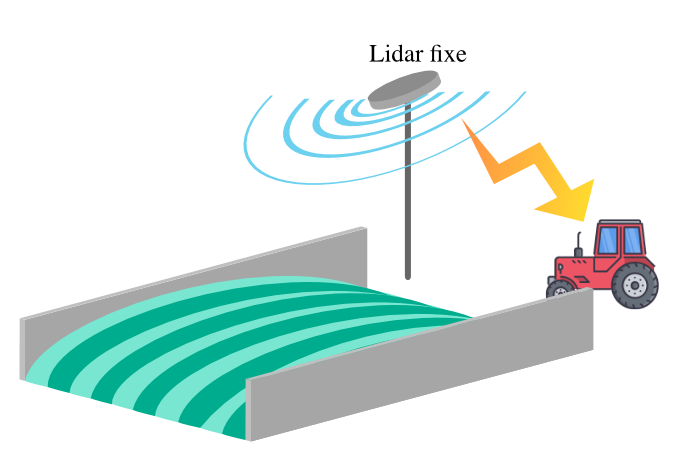
\includegraphics[width=0.7\linewidth]{img/LidarFixe}
	\caption[]{Configuration avec Lidar fixe}
	\label{fig:lidarfixe}
\end{figure}


Ce système est déjà en exploitation par les clients de Tellus Environment et un retour d'expérience à été effecuté auprès des opérateurs. Le principal défaut remonté de l'équipement lors son exploitation est le temps d'installation du Lidar dans une des coins du silos qui prend en temps certain. Les contraintes en temps des intervenants autour d'un tassage de silo ne sont pas compatibles avec le déploiment d'un instrument sensible comme un Lidar.

\paragraph{} Un besoin supplémentaire a été de plus exprimé: une mesure précise du volume d'ensilage tassé dans le silo doit pouvoir être fournie. 

\paragraph{La solution à ces demandes} envisagée par Tellus Environment est donc de purement et simplement supprimer cette étape d'installation en montant le Lidar directement sur le tracteur de tassage, et de faire évoluer le logiciel de manière à ce qu'il puisse estimer l'état de surface de l'ensilage tassé ainsi que le volume d'ensilage tassé.

\begin{figure}[H]
	\centering
	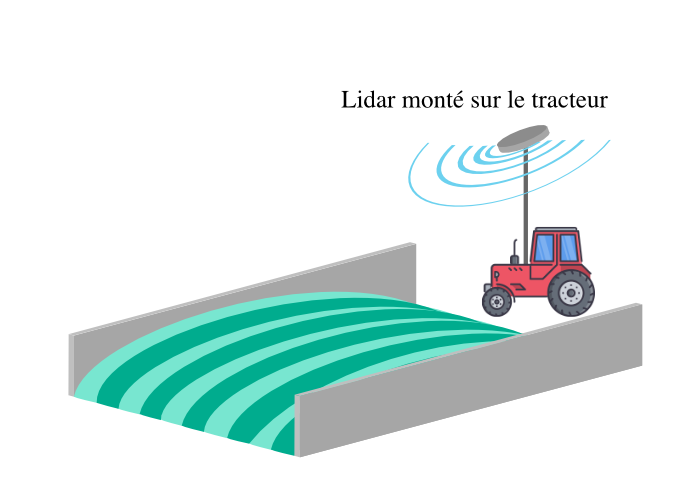
\includegraphics[width=0.7\linewidth]{img/LidarMobile}
	\caption{Configuration avec Lidar monté sur le tracteur}
	\label{fig:lidarmobile}
\end{figure}


\section{Objectifs du projet de pré-stage}
Le projet de pré-stage a pour objectif principal d'enquêter sur les techniques de mesure précise d'un tas d'ensilage à partir de capteurs montés sur une plateforme mobile, en vue de le les mettre en oeuvre lors du stage.

Les sujets à aborder seront les suivants:
\begin{enumerate}[label=\textbf{\arabic*.}]
	\item \textbf{Notions sur les chantiers d'ensilage:} l'objet de cette partie est de déterminer précisement ce qui constituera l'environnemnent opérationnel du système V2, à savoir les chantier d'ensilage. Nous étudierons pourquoi les silos sont nécessaires à une exploitation, les moyens engagés sur un chantier d'ensilage et les critères de qualité sur la conduite de ces chantiers. 
		
	\item \textbf{Les Capteurs pour les systèmes mobiles:} généralités sur les différents types de capteurs succeptibles d'être utilisés sur le projet.
	
	\item \textbf{Analyse de la solution existante:} cette partie s'attachera à analyser en détail la version 1 de la solution, en vue d'en dégager les points forts et les points faibles.


	\item \textbf{Les Outils Importants:} détecter les outils qui se réveleront nécessaires à la bonne conduite du stage:
	\begin{itemize}
		\item Plateforme Robot OS: système d'exploitation sous lequel la solution sera déployée.
		\item Localisation, Cartographie, SLAM: les outils pour l'implémentation d'un système "Simultaneous Localization And Mapping"
		\item Mesurer le tassage: les outils mathématiques pour reconstituer en 3D le tas d'ensilage à partir de relevé issus d'un LIDAR
		\item Prototypage et mise en oeuvre: les différents outils qui permettront de modéliser le système, monter et tester des prototype simulés ou en grandeur.
	\end{itemize}
	
	\item \textbf{Application numérique:} mettre en oeuvre un algorithme de détection d'un mur à partir d'un nuage de points.
	
	\item \textbf{Critères SMART pour le projet de stage:} évaluer les facteurs de succès du stage sur la base des critères SMART.
\end{enumerate}

\chapter{L'ensilage de maïs en silo}

L'objectif de ce chapitre est d'introduire l'environnement opérationnel dans lequel le produit final sera déployé, à savoir les chantiers d'ensilage de maïs sur les exploitations d'élevage agricole.

\paragraph{}

Dans une exploitation d'élevage agricole, l'ensilage a pour but  de stocker des fourrages de manière à en permettre la conservation de nourriture animal, à longue durée et en grande quantité.


\section{Les fourrages: importance économique}

\paragraph{La nourriture: poste de charges le plus important pour une exploitation agricole} Pour un élevage agricole, la nourriture animale représente la charge financière la plus importante pour tout élevage agricole. Selon \cite{noauthor_alimentation_2017} :"Les coûts liés à la culture des surfaces fourragères et aux achats de produits d'alimentation représentent plus de 50\% du prix de revient des animaux."



\paragraph{Les fourrages: un moyen bon marché pour nourrir les herbivores.} Toujours selon \cite{noauthor_alimentation_2017}, un moyen efficasse de réduire les coûts liés à l'alimentation animale est d'éviter au maximum l'achat de produits extérieurs à la ferme, en pratiquant le paturage dans les prairies naturelles ou semées, ou alors en amenant aux animaux du fourrage récolté sur la ferme, par exemple.

\paragraph{} L'abondance de ces produits disponibles en ferme variant selon les saisons et devenant rares en hiver, il est nécessaire pour un éleveur d'avoir à disposition des aliments stockés en quantité suffisante pour cette période. De plus ces aliments doivent être conservés dans des conditions d'hygiène  telles qu'ils soient toujours comestibles pour les animaux, et les garder en bonne santé.

\paragraph{} Selon \cite{noauthor_ensilage_2018} et \cite{cuvelier_lalimentation_2015}, la manière la plus courante de stocker l'alimentation d'animaux herbivores est la technique de l'ensillage.


\section{Principes de l'ensilage}

Selon \cite{noauthor_ensilage_2018} et \cite{cuvelier_lalimentation_2015}, l’ensilage est un système de conservation des fourrages par fermentation anaérobique dans un silo. Des bactéries transforment les sucres solubles en acides organiques (principalement de l'acide lactique et de l’acide acétique). Ces produit rendent l'ensilage acide, ce qui le stérilise et permet sa conservation à long terme.

\subsection{Fermentation Lactique}
Selon \cite{noauthor_ensilage_2018}, la principale fermentation en jeu dans les ensilages de maïs est la fermentation lactique. Comme indiqué dans \cite{noauthor_fermentation_2018} :“la \textbf{fermentation lactique}, ou \textbf{lacto-fermentation}, est un mode de fermentation (production d'énergie anaérobie) qui, en présence de glucides et de bactéries spécifques (les ferments lactiques), induit la formation d'acide lactique.

La production d'acide lactique provoque une acidification du milieu, qui permet l'élimination d'autres bactéries, éventuellement pathogènes."

\paragraph{Réaction chimique:} La fermentation anaérobie a lieu, comme indiqué dans \cite{noauthor_fermentation_2018}, en absence d'oxygène. La réaction chimique combine le glucose, l'adénosine diphosphate (ADP) et le phophate inrganique (Pi) pour produire de l'acide lactique ($C_3H_6O_3$) et de l'adénosine triphosphate (ATP), comme indiqué dans l'équatin chimique \ref{reacchim}.

\begin{equation}
	C_6H_{12}O_6 + 2 ADP + 2 Pi \rightarrow 2 C_3H_6O_3 + 2 ATP
	\label{reacchim}
\end{equation}


\paragraph{Stérilisation et conservation:} Selon \cite{noauthor_fermentation_2018} Les légumes portent en leur surface des micro-organismes qui laissés à l'air libre provoquent leur putréfaction. En l'absence d'air et en présence d'une légère quantité de sel qui inhibe les autres ferments, les ferments lactiques prennent le dessus. Ces bactéries se développent en assimiant les glucides présents dans les légumes et les transforment en acide lactique. 

\paragraph{}Au fur et à mesure de la progession du processus, la concentration d'acide lactique augmentant, le jus devient de plus en plus acide et neutralise le développement de la putréfaction. Lorsque que le milieu atteint une acidité suffisante (pH autour de 4), les bactéries lactique deviennent elles-mêmes inhibées et la fermentation s'arrête. Le produit devient stable, ce qui permet une longue conseration.

\paragraph{}Toujours selon \cite{noauthor_fermentation_2018}, la fermentation lactique est utilisée depuis longtemps pour préparer une grande variété d'aliments, y compris destinés à une consommation humaine. De nombreux fruits et légumes peuvent être consommés fermentés, comme le chou (choucroute, kimchi), les carottes, la betterave, les cornichons, le citron, les olives, etc. Les yaourts, les faisselles et d'autres poduits laitiers frais "rustiques" (lait ribot) utilisent le principe de la fermentation lactique. 

\paragraph{}Selon \cite{maciejewski_productions_2015}La fermentation lactique est donc aussi utilisée pour la conservation des fourrages annuels, comme le maïs ensilage, la betterave fourragère et le sorgho fourragé sont conservés selon des procédés basés sur la fermentation lactique.

\subsection{Conservation des fourrages annuels}

Il existe plusieurs méthodes d'ensilage, c'est à dire de méthodes de conservation des fourrages annuels basées sur la fermentation lactique. Selon \cite{noauthor_ensilage_2018} elles sont au nombre de trois:

\paragraph{Le "Haylage":} cette technique  consiste en l'empilement vertical du fourrage dans des silos-tours limitant le contact avec l'air. L'anaérobiose est assurée par l'épaisseur de l'ensemble.
Cette méthode qui requiert des investissements lourds (silo, soufflerie, mécanisme de désillage) est principalement utilisée au Etats-unis où elle a été mise au point. Elle est peu fréquente en Europe.

\paragraph{L'Enrubannage:} cette méthode consiste au stockage du fourrage dans des balles rondes résultant du déroulage d'un film plastique autour de chaque botte . L'anaérobiose résulte de l'étanchéité à l'air du film plastique.


\paragraph{Ensilage en silo couloir} Cette technique est la plus utilisée. Le fourrage est d'abord haché en particules d'environ un centimètre de long, puis stocké à plat en couches successives, sur une aire bétonnée entre deux murs. Il est compacté au fur et à mesure à l'aide de trcteurs afin d'expulser le maximum d'air intersticiel. Il est enfin mi en anaérobiose définitive par recouvrement à l'aide d'une bâche de polyéthylène lestée.

\paragraph{} La même technique peut être utilisée lorsqu'on ne dispose pas de murs limitant le silo. On parle alors de \textbf{silo taupinère}, fréquemment utilisé pour la pulpe de bettrave.

\section{Ensilage en silo couloir: mise en oeuvre}

Un chantier d'ensilage consiste à la récolte et la mise en silo immédiate du fourrage en vue de le mettre à fermenter. Il s'agit donc d'un chantier à plusieurs postes qui tournent en parallèle et à flux tendu.

\subsection{Le chantier d'ensilage de }

\paragraph{Vue d'ensemble :} 

\paragraph{Les différents postes}
\subparagraph{Fourrageuse:} La fourrage récolte le fourrage en champ, le découpe en morceaux d'environ 1 centimètre et le déverse dans la remoque de la navette, tout cela de manère continue;
\subparagraph{Navette:} La navette suit la fourrageuse dans le champ le temps que celle-ci remplisse sa remorque de fourrage. Ue fois la remorque remplie, la navette se rend au silo, dépose le fourrage au pied du silo et retourne auprès de la fourrageuse. Il peut y avoir plusieurs navettes sur un même chantier.
\subparagraph{Tracteur étaleur:}ce tracteur sert à étaler dans le silo le fourrage déversé par la navette.
\subparagraph{Tracteur tasseur:}ce tracteur sert à tasser le fourrage; c'est une tâche précise et non sans danger (risque de chute et de renversement). Son rôle est primordial dans la bonne exécution du tassage et le plus important facteur pour obtenir une fermentation de qualité.

\subsection{Méthodologie du remplissage et de tassage du silo}

Le remplissage et le tassage du silo est effectué de telle manière à ce que le fourrage soit tassé uniformément sur toute son épaisseur. En vue de réduire la surface de plastique nécessaire pour recourvir ent!èrement le  fourrage, la forme du silo "couloir" va être plutôt ramassée qu'en longueur. Les murs sont présents pour permettre au fourrage de monter en hauteur et favoriser ainsi l'anaérobie.
\newline

Les silos ont généralement une taille de quelques dizaines de mètres sur un peu moins de large. La hauteur des murs est de 1,5m à 2,5m.

\paragraph{Préparation du silo} Le silo est initalement préparé, les murs et le sol nettoyés. Une bache propre est disposée contre les murs.

\paragraph{Etalement initial:} La première couche d'ensilage est étalée à une épaisseur de 50 cm. Le tracteur tasseur passe ensuite pour obtenir une épaisseur finale d'environ 30 centimetres pour cette première couche. Une attention particulère est apportée pour tasser les cotés du silo.

\paragraph{Etalements successifs} Les couches suivantes sont ensuite étalées à 20cm d'épaisseur et aussitôt tassés à 10cm. Encore une fois les côtés du silo sont tassés avec attention car la hauteur augmentant, les tracteurs se trouvent très hauts par rapport au sol et risquent de basculer.

\paragraph{Isolation hermétique:} Une fois le remplissage et le tassement complétés, le silo est fermé hermétiquement par des baches en polyérhylène lesté. Il est laissé à fermenter à fermenter pendant 6 à 8 semaines.

\paragraph{Les paramètres cibles: } D'après \cite{trachsler_planifier_nodate}, il faut remplir rapidement et bien compacter. Il faut obtenir plus de 200kg de MS (matière sèche) par m$^3$. On peut atteindre 270 kg de MS par m$^3$ dans un silo-couloir si le fourrage est bien tassé.


\subsection{risques d'un tassage mal effectué}
Toujours d'après \cite{trachsler_planifier_nodate}, dans les silos mal compactés avec moins de 160 kg de MS par m$^3$ d'ensilage, le silo contient peu de fourrage et l'ensilage est instable. Les mesures montrent que l'oxygène pénètre dans ce cas jusqu'à 2,5m à l'intérieur du tas de fourrage. 

\paragraph{Conséquences} un silo mal compacté a généralement les conséquences suivantes pour un éleveur:

\begin{itemize}
	\item la fermentation est partielle, ce qui rend l'ensilage instable (la fermentation peut reprendre de manière non contrôlée)
	\item le niveau d'acidité cible n'est pas atteint, ce qui implique une stérilisation moindre
	\item le fourrage est beaucoup plus succeptible de pourrir.
	\item des pertes importante d'ensilage seront à prévoir car le produit sera impropre à la consommation animale.
\end{itemize}

\paragraph{Mesurer le tassage:} La mesure du tassage du silo en cours de chantier n'est pas simple. Il faut tout d'abord prendre en compte la teneur en MS du fourrage, avoir une idée du tonnage récolté, et évaluer le volume effectif de fourrage tassé dans le silo.
\newline

De plus, la réaction mécanique du fourrage au tassage va beaucoup varier en fonction du temps d'humidité du fourrage, et aussi de sa nature. Il faudra plus tasser si le fourrage est relativement plus humide, il peut y avoir un comportement légèrement elastique qui fait que le tassage se réduit si le tracteur ne passe pas plusieur fois en peu de temps. 

Tous ces facteurs font que le tassage est difficile à estimer sur le chantier.

\section{Préparation et la conduite du chantier}

\subsection{Les différents types d'intervenant}
Propriétaires, Groupement agricoles, prestaires de services

\subsection{Gestion de production}
\paragraph{cible de production} prévision de consommation: $x$ kg par jour et par bête $\rightarrow$ quantité d'ensilage à produire.

\paragraph{éviter la surproduction}

\paragraph{permettre la mise en valeur du maïs sur pied restant}




\section{Conclusion}
Nous avons vu que le tassage de silo est une activité stratégique pour une exploitation, qui requiert des moyens lourds, de la planification. C'est de plus une activité très technique, qui est effectuée en parallèle de la récolte, en flux tendu et dont le résultat peut être rendu aléatoire si il n'est pas effectué avec méthode.

\chapter{Solution Actuelle à Améliorer}
Le présent chapitre s'attache à présenter la première version du système de mesure de tassage de silo mis en place par Tellus Enviroement.
\section{Objectifs initiaux de la version V1}
L'objectif initial de ce système est d'apporter une aide à la conduite du tassage sur le chantier d'ensilage en indiquant quelles partie du tassage doit être tassé en priorité.
\newline

Il n'y pas de mesure explicite de la taille du tas de fourrage, ni de calcul du volume. Le LIDAR effectue une mesure mesure relative de la hauteur du fourrage et in

\section{Présentation de solution}
\subsection{Architecture de la solution}

L'architecture de la première solution peut être représentée par le schéma \ref{fig:archigenv1} ci-dessous.

\begin{figure}[H]
	\centering
	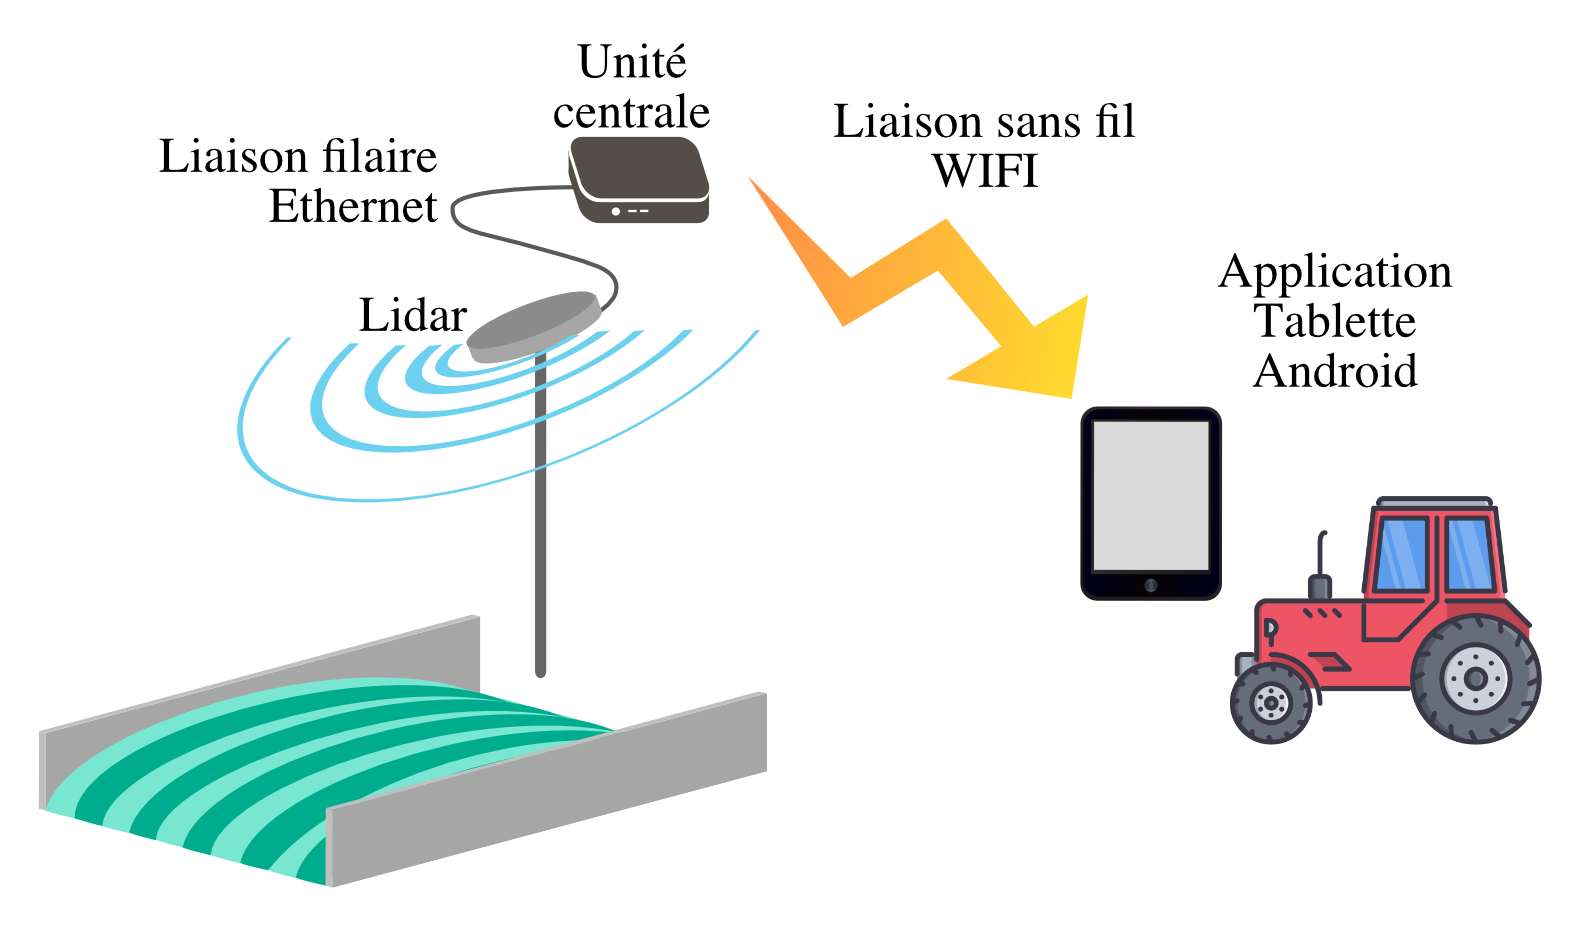
\includegraphics[width=0.7\linewidth]{img/ArchiGenV1}
	\caption{Architecture de la solution V1}
	\label{fig:archigenv1}
\end{figure}


\subsection{Les sous-systèmes}
Le système est composé des éléments suivants:

\begin{enumerate}
	\item \textbf{LIDAR:} Il s'agit d'un équipement à base de laser qui effectue des mesures très rapides et précise du tas de fourrage. Il est situé à 7m de hauteur de manière à bien dominer l'ensemble du silo, et de manière à ce qu'il n'y ai pas d'effet d'horizon qui cache un partie du silo. Pour cela il monté sur un mat téléscopique, lui même maintenu par un robuste trépied.
	
	\item \textbf{Unité centrale:} Réliée au Lidar au moyen d'une connexion filaire ethernet, l'unité centrale met en oeuvre le système d'exploitation "Robot OS". Il execute un programme dédié qui collecte les données générées par le Lidar. Ce programme exploite ces informations pour mesurer avec précision les variations de hauteur du tas de fourrage, et générer une image indiquant les zones à tasser en priorité.
	
	\item \textbf{Application tablette Android:} Relié à l'unité centrale par une liaison sans fil WIFI, cette application récupère l'image générée par celle-ci et la présente au conducteur du tracteur.
\end{enumerate}

\section{Points faibles et axes d'amélioration}
Selon Tellus Environment, cette première version du système a été utilisé sur environ une dizaine de chantier dans le courant de l'année 2017, et un retour d'expérience a permis de mettre en évidence plusieurs points faibles et axes d'amélioration.

\subsection{Complexité de mise en oeuvre}

Du fait de son architecture, la mise en oeuvre requiert le déploiement de deux équipements distincts pour être opérationnel:

\begin{itemize}
	\item la \textbf{tablette Android} dans le tracteur pour afficher la carte du tas de fourrage
	\item le bloc \textbf{LIDAR + Unité centrale} qui est perché en haut d'un mat de 7m de hauteur.
\end{itemize}

Cette configuration induit plusieurs difficultés dans la mise en oeuvre du système qui peuvent porter préjudice à son utilisabilité.

\paragraph{Installation délicate du Lidar:} En début de chantier le block LIDAR + Unité Centrale doit être positionné et orienté de manière à pouvoir couvrir la totalité du silo. Il faut donc un surface relativement stable à proximité directe du silo pour installer le trépied qui maintient le mat téléscopique.

\paragraph{} Ensuite il faut positionner le Lidar en direction et inclinaison. Le support du Lidar en haut du mat n'étant pas motorisé, il faut donc effectuer ce réglage "à la main", soit en montant sur une échelle pour y accéder et viser à l'oeil nu, soit en vérifiant le cadrage sur la tablette Android et descendre le cas échéant le lidar pour modifier le cadrage, puis le remonter encore, jusqu'à obtenir un réglage satisfaisant.

\paragraph{} L'installation du Lidar est donc délicate, et est à l'usage consommatrice de temps. Or le temps est une denrée précieuse sur un chantier d'ensilage, et certains opérateurs ont une exigence forte sur la rapidité de déploiement de leurs équipements. La perception de ces opérateurs est donc que cette exigence n'est pas complètement satisfaite par le système dans sa forme actuelle.


\paragraph{Connectivité WIFI peu adaptée à l'environnement du chantier: } Tout au long du chantier, la connectivité entre la tablette Android et l'unité centrale est assurée au moyen d'un réseau sans fil WIFI. Or, un réseau WIFI requiert lui aussi une configuration initiale qui peut être problématique et consommatrice de temps.

\paragraph{} De plus la porté d'un réseau WIFI, dans les meilleur conditions sera de quelques dizaines de mètres. L'ordre de grandeur de cette porté est donc de l'ordre de la taille des silos. Ceci implique que, si le tracteur équipé de la tablette est à l'entrée du silo opposé à celle où est installé le LIDAR, les conditions de communication sont loin d'être optimales.

\paragraph{} Il en résulte donc des pertes de connexion, qui font qu la tablette n'est plus en mesure d'afficher les informations de l'état de tassage du silo. Le conducteurd'intervenir manuellement pour ré-établir la connexion. 


\subsection{Limitation du système}
\paragraph{Informations limitées:} Le système dans sa forme actuelle ne fourni en fait qu'une seule information: l'état de tassage du silo, c'est dire une information sur la différence de hauteur sur l'ensemble du silo. Il n'y a pas de mesure numérique précise.

\paragraph{} Une demande des opérateurs est donc de faire évoluer le système de manière à ce qu'il permette de mesurer précisement le volume du fourrage ensilé.

\paragraph{Pas de calibrage:} Le système ne fait aucune calibration de ses mesures en fonction du chantier. Ceci empêche de faire évoluer à bas coût le système pour ajouter des fonctionnalités qui ajouterai de la valeur au système.

\paragraph{Lidar placé très prés du silo:} Pour apporter des informations utiles et exploitables aux les tasseurs, le LIDAR doit être placé le plus près possible du silo. Or cela veut dire que les tracteurs doivent passer dans certains cas très prés du mat sur lequel repose le Lidar, au risque de le faire basculer. Les tracteurs doivent donc apporter une attention particulière pour préserver le Lidar, ce qui les gène dans leur travail.

\subsection{Axes d'améliorations pour la V2}

Sur la base des points faibles et limitations listés ci-dessus, Tellus Environment envisage donc de faire évoluer la solution de manière à supprimer ses défauts majeurs et lui permettre d'obtenir des informations précises et chiffrées sur l'état de tassage du silo.

\paragraph{} Les facteurs limitants sont les suivants:

\begin{itemize}
	\item des éléments répartis à différents endroits du chantier requiert un réseau sans fil peu fiable dans l'environnement d'un chantier d'ensilage
	\item La configuration initiale délicate du Lidar est consommatrice de temps
	\item Le Lidar à proximité immédiate du silo gène les tracteurs.
\end{itemize}

\paragraph{Supprimer les facteurs limitants de mise en oeuvre:} Monter tous les éléments directement sur la tracteur permet d'éliminer tous les facteurs limitants. 
En remplaçant le lidar fixe à proximité du silo par un ou plusieurs Lidars montés directement sur le tracteur, et donc en montant l'unité centrale elle aussi sur le tracteur, nous pouvons relier tous les sous-système par un cablage fixe à bord du tracteur tasseur.

\paragraph{} Cette configuration élimine le besoin de mettre en oeuvre un réseau sans fil. Elle élimine aussi la nécessité de déployer un appareil dont la mise en place est délicate en début de chantier, puisque le tracteur sera équipé en permanence des capteurs. 

\paragraph{Obtenir des informations supplémentaires sur l'état de tassage:} Il est par contre évident qu'obtenir une vue d'ensemble de l'état de tassage du silo à partir d'une plateforme mobile qui de plus aura une vue parcellaire du silo à chaque instant requièrera un algorithme de calcul bien plus complexe que dans la première version du système.

\paragraph{} En effet, le nouveau système devra être en mesure de reconstituer la scène du chantier dans sa globalité à partir de mesures fragmentaires.

\paragraph{} Par contre un système qui atteindrait cette performance sera en mesure de fournir des informations à la fois précises et nombreuses aux utilisateurs, et ce à un coût relatif moindre. L'une de ces mesures, le \textbf{volume du tas de fourrage}, sera immédiate.
\newpage

\section{Conclusions}

\paragraph{}Nous avons vu que le premier système permettait de fournir aux utilisateurs une mesure de l'état de tassage d'un fourrage dans un silo horizontal (couloir ou semi-enterré).

\paragraph{}Nous avons vu que ce système, bien qu'opérationnel, était sujet à des défauts qui requièrent des modifications.

\paragraph{}Ces modifications impliquent le développement d'un procédé qui permette à partir d'un ensemble de mesure partielles, potentiellement à des instant différents, de reconstituer virtuellement le chantier dans son ensemble. Cette reconstitution devra être faite de manière \textbf{autonome}, en \textbf{temps-réel} et avec \textbf{précision}.

\paragraph{}Les outils mathématiques et technologiques seront ceux des systèmes mobiles autonomes, ce seront ceux de la \textbf{robotique}.






\part{Outils Importants }

\chapter{Détecteurs en Robotique}

Notre projet va s'attacher à mesurer un volume d'ensilage à partir d'une plateforme mobile. Cette plateforme doit donc être en mesure de déterminer sa propre position dans le théatre d'opération, de mesurer le silo et de mesure la surface d'ensilage qui y est tassée.

\paragraph{} Ces informations sont recueillies à l'aide de capteurs dont la mise en oeuvre sera une partie majeure du projet.

\section{Notions sur les capteurs}

\subsection{Informations fournies par un capteur de présence}

Mesure de grandeur, fréquence, précision / marge d'erreur.

\paragraph{Portée}
\paragraph{Ouverture} Ouverture en largeur, ouverture en hauteur

\paragraph{Distance, gisement, azimuth}




\section{Les capteurs de position}

\subsection{Odométrie}
L'objet de l'odométrie pour un système mobile est de détecter ses propres déplacements afin de déterminer sa nouvelle position sur la base de capteurs apropriés.


Par exemple, une système mobile à roue peux compter le nombre de tours de roue effectués pour calculer la distance parcourrue.


\subsection{Centrales inertielles}

\subsection{GPS}

\section{Les détecteurs de type "Direction et Portée"}

\subsection{Principes}

\paragraph{Mesures}

\paragraph{Modes d'exploitation}
modes de balayage

\subsection{Les différents types de capteur "Direction et Portée"}

\section{Les capteurs de type "Direction"}
Capteur qui ne sont en mesure de fournir une information que sur la direction de l'objet détecté, sans pouvoir fournir d'information intrinsèque quand à la distance de l'object détecté.

\subsection{Détecteur de présence}

\subsection{Vision par Ordinateur}, analyse d'image, etc

\section{Les détecteurs de type "Portée seulement"}

Détecteurs qui ne fournissent que la portée d'un objet détecté, sans pouvoir fournir d'information précise sur la direction de l'objet en question.

\chapter{Localisation, Cartographie, SLAM}
\section{Positionnement du problème}

\paragraph{Localisation requiert une carte}

\paragraph{Cartographier requiert de connaître sa position}

\paragraph{SLAM permet de résoudre cette problématique "Oeuf et poule"} en mettant à disposition des outils permettant d'exploiter au mieux les informations issues des différents types de capteurs disponibles.

\paragraph{Localisation, vecteur d'état: } système de coordonnées, vecteur d'état.


\section{Maintenir de le vecteur d'état}

\paragraph{Mise en place de la boucle de rafraichissment, filtres de Kalman}

\paragraph{Selectionner des points de repère, les maintenir}

\section{Reconstituer l'environnement}


\chapter{Mesurer le tassage}

\section{Modéliser une surface en 3D}

\section{Calculer le volume à partir d'une surface 3D mesurée}


\chapter{Prototypage}
\section{Prototypage Scientifique des Algorithmes}
\subsection{Matlab}
\subsection{Python}
\section{Prototype de mise en œuvre}
\subsection{Plateforme ROS}
\subsection{Mise en oeuvre en C et/ou C++}

\part{Application Numérique}

\chapter{Application Numérique}
L'objectif de cette partie est de concevoir et mettre en oeuvre un algorithme de détection de forme à partir d'un nuage de points, pouvant être issu d'un capteur de type "portée et direction".

\begin{enumerate}
\item
Produire des données de référence à partir de modèle de structure 3D connus.
\item
Introduire bruit gaussien sur les points, de manière à produire un nuage de points bruité
\item
Développer un technique d'inversion permettant de détecter la forme
et les dimensions des structures à partir des nuages de points
bruités
\item
Evaluer les marges d'erreur des modèles inversés
\item
Dégager les axes de progression en terme de performance de calcul:
l'objectif est d'obtenir des outils qui produisent des résultats en
quelques secondes.
\end{enumerate}

\part{Conclusions du Projet Préliminaire au Stage}
  
\chapter{Objectifs SMART du Stage}
\chapter{Conclusion}

\begin{appendix}
\chapter{Sujet de stage}
Le sujet de stage est inclus dans les deux pages suivantes.
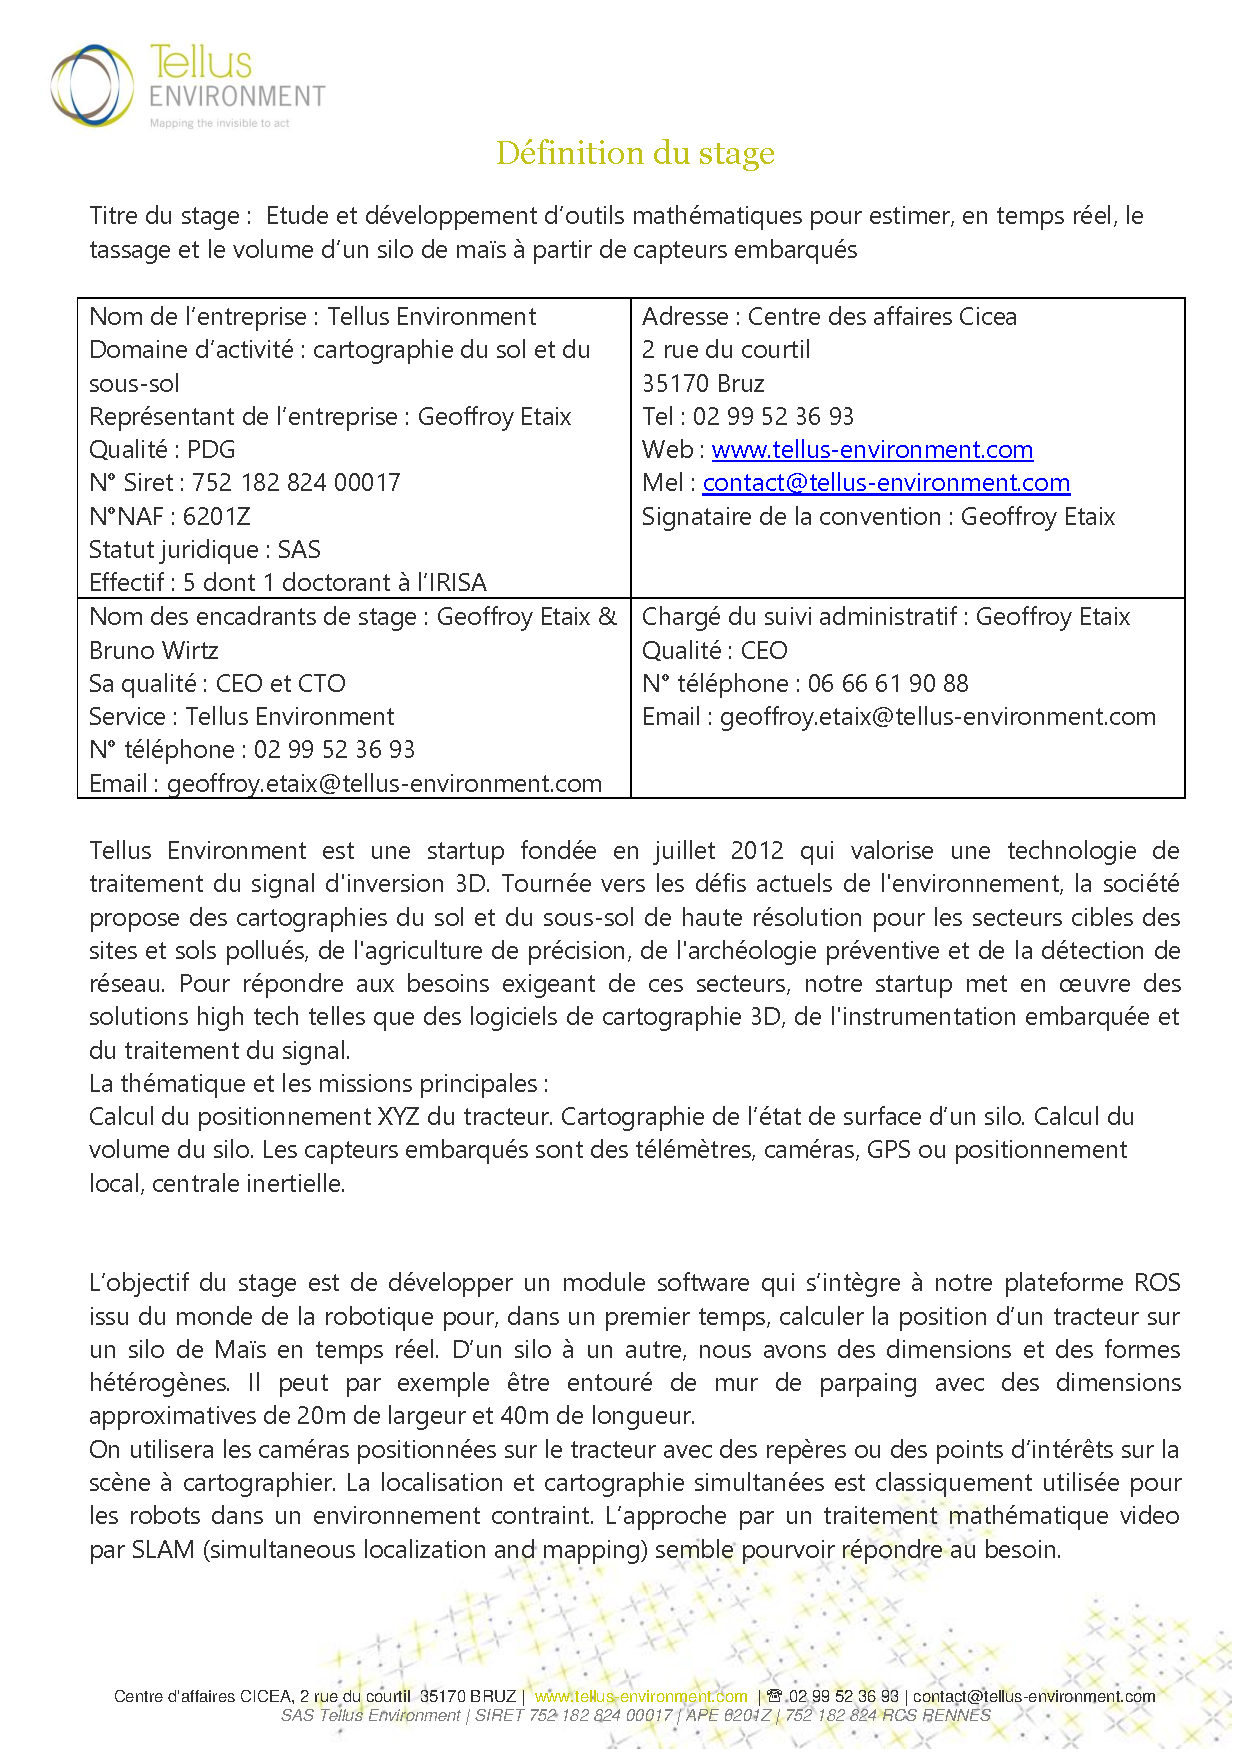
\includepdf[pages={1,2},pagecommand={}]{sujetstage}
\end{appendix}

\bibliographystyle{plain}
\bibliography{biblio}

\end{document}
